\renewcommand*{\arraystretch}{1.1}

\subsection*{Interactive / complex / 14}
\label{section:interactive-complex-read-14}

% change \emph{} to use sans-serif font
\let\oldemph\emph
\renewcommand{\emph}[1]{{\footnotesize \sf #1}}

\renewcommand{\currentQueryCard}{14}
\marginpar{
	\raggedleft
	\vspace{0.22ex}

    \queryRefCard{interactive-complex-read-01}{Interactive}{1}\\
    \queryRefCard{interactive-complex-read-02}{Interactive}{2}\\
    \queryRefCard{interactive-complex-read-03}{Interactive}{3}\\
    \queryRefCard{interactive-complex-read-04}{Interactive}{4}\\
    \queryRefCard{interactive-complex-read-05}{Interactive}{5}\\
    \queryRefCard{interactive-complex-read-06}{Interactive}{6}\\
    \queryRefCard{interactive-complex-read-07}{Interactive}{7}\\
    \queryRefCard{interactive-complex-read-08}{Interactive}{8}\\
    \queryRefCard{interactive-complex-read-09}{Interactive}{9}\\
    \queryRefCard{interactive-complex-read-10}{Interactive}{10}\\
    \queryRefCard{interactive-complex-read-11}{Interactive}{11}\\
    \queryRefCard{interactive-complex-read-12}{Interactive}{12}\\
    \queryRefCard{interactive-complex-read-13}{Interactive}{13}\\
    \queryRefCard{interactive-complex-read-14}{Interactive}{14}\\
}


\noindent\begin{tabularx}{\queryCardWidth}{|>{\queryPropertyCell}p{\queryPropertyCellWidth}|X|}
	\hline
	query & Interactive / complex / 14 \\ \hline
%
	title & Weighted/unweighted paths
 \\ \hline
%
	pattern & \hfill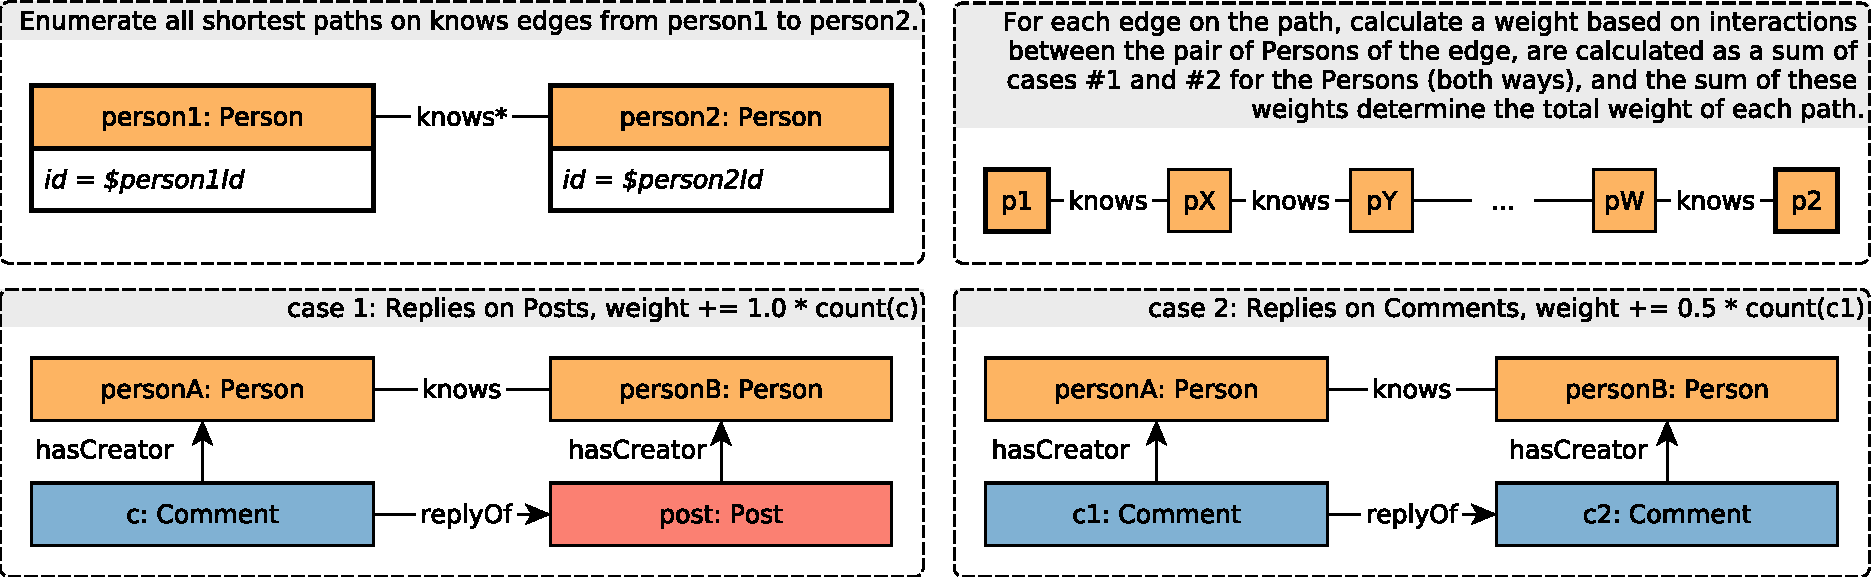
\includegraphics[scale=\patternscale,margin=0cm .2cm]{patterns/interactive-complex-read-14}\hfill\vadjust{} \\ \hline
%
	desc. & Given two Persons, find all (unweighted) shortest paths between these
two Persons, in the subgraph induced by the Knows relationship. Then,
for each path calculate a weight. The nodes in the path are Persons, and
the weight of a path is the sum of weights between every pair of
consecutive Person nodes in the path. The weight for a pair of Persons
is calculated such that every reply (by one of the Persons) to a Post
(by the other Person) contributes 1.0, and every reply (by ones of the
Persons) to a Comment (by the other Person) contributes 0.5. Return all
the paths with shortest length, and their weights. Do not return any
rows if there is now path between the two Persons.
 \\ \hline
%
	
		params &
		\innerCardVSpace{\begin{tabularx}{\attributeCardWidth}{|>{\paramNumberCell}c|>{\varNameCell}M|>{\typeCell}m{\typeWidth}|Y|} \hline
		$\mathsf{1}$ & person1.id
 & ID
 &  \\ \hline
		$\mathsf{2}$ & person2.id
 & ID
 &  \\ \hline
		\end{tabularx}}\innerCardVSpace \\ \hline
	
%
	
		result &
		\innerCardVSpace{\begin{tabularx}{\attributeCardWidth}{|>{\resultNumberCell}c|>{\varNameCell}M|>{\typeCell}m{\typeWidth}|>{\resultOriginCell}c|Y|} \hline
		$\mathsf{1}$ & {[}Person.id{]} & {[}ID{]} & C &
				Identifiers representing an ordered sequence of the Persons in the path
 \\ \hline
		$\mathsf{2}$ & weight & 64-bit Float & C &
				 \\ \hline
		\end{tabularx}}\innerCardVSpace \\ \hline
	
%
	
		sort		&
		\innerCardVSpace{\begin{tabularx}{\attributeCardWidth}{|>{\sortNumberCell}c|>{\varNameCell}M|>{\directionCell}c|Y|} \hline
		$\mathsf{1}$ & weight
 & $\desc
$ & The order of paths with the same weight is unspecified
 \\ \hline
		\end{tabularx}}\innerCardVSpace \\ \hline
	%
	%
	CPs &
	\multicolumn{1}{>{\raggedright}l|}{
		\chokePoint{3.3}, 
		\chokePoint{7.2}, 
		\chokePoint{7.3}
		} \\ \hline
	%
	relevance &
		\small This query looks for a variable length path, starting at a given Person and finishing at an another given Person. This
is a more complex query as not only requires computing the path length, but returning it and computing a weight.
To compute this weight one must look for smaller sub-queries with paths of length three, formed by the two Persons
at each step, a Post and a Comment.
 \\ \hline%
\end{tabularx}
\queryCardVSpace

% change \emph back to the old one
\renewcommand{\emph}[1]{\oldemph{#1}}